\item \points{15} {\bf Logistic Regression: Training stability}

In this problem, we will be delving deeper into the workings of logistic
regression. The goal of this problem is to help you develop your skills
debugging machine learning algorithms (which can be very different from
debugging software in general).

We have provided an implementation of logistic regression in
\texttt{src/stability/stability.py}, and two labeled datasets $A$ and $B$ in
\texttt{src/stability/ds1\_a.csv} and \texttt{src/stability/ds1\_b.csv}.

Please do not modify the code for the logistic regression training algorithm
for this problem. First, run the given logistic regression code to train two
different models on $A$ and $B$. You can run the code by simply executing
\texttt{python stability.py} in the \texttt{src/stability} directory.

\begin{enumerate}

  \item \subquestionpoints{2}
What is the most notable difference in training the logistic regression model
on datasets $A$ and $B$?


\ifnum\solutions=1 {
  %
\documentclass{article}

\usepackage{graphicx}

\newcommand{\di}{{d}}
\newcommand{\nexp}{{n}}
\newcommand{\nf}{{p}}
\newcommand{\vcd}{{\textbf{D}}}

\usepackage{nccmath}
\usepackage{mathtools}
\usepackage{graphicx,caption}
\usepackage{enumitem}
\usepackage{epstopdf,subcaption}
\usepackage{psfrag}
\usepackage{amsmath,amssymb,epsf}
\usepackage{verbatim}
\usepackage[hyphens]{url}
\usepackage{color}
\usepackage{bbm}
\usepackage{listings}
\usepackage{setspace}
\usepackage{float}
\usepackage{natbib}
\definecolor{Code}{rgb}{0,0,0}
\definecolor{Decorators}{rgb}{0.5,0.5,0.5}
\definecolor{Numbers}{rgb}{0.5,0,0}
\definecolor{MatchingBrackets}{rgb}{0.25,0.5,0.5}
\definecolor{Keywords}{rgb}{0,0,1}
\definecolor{self}{rgb}{0,0,0}
\definecolor{Strings}{rgb}{0,0.63,0}
\definecolor{Comments}{rgb}{0,0.63,1}
\definecolor{Backquotes}{rgb}{0,0,0}
\definecolor{Classname}{rgb}{0,0,0}
\definecolor{FunctionName}{rgb}{0,0,0}
\definecolor{Operators}{rgb}{0,0,0}
\definecolor{Background}{rgb}{0.98,0.98,0.98}
\lstdefinelanguage{Python}{
numbers=left,
numberstyle=\footnotesize,
numbersep=1em,
xleftmargin=1em,
framextopmargin=2em,
framexbottommargin=2em,
showspaces=false,
showtabs=false,
showstringspaces=false,
frame=l,
tabsize=4,
% Basic
basicstyle=\ttfamily\footnotesize\setstretch{1},
backgroundcolor=\color{Background},
% Comments
commentstyle=\color{Comments}\slshape,
% Strings
stringstyle=\color{Strings},
morecomment=[s][\color{Strings}]{"""}{"""},
morecomment=[s][\color{Strings}]{'''}{'''},
% keywords
morekeywords={import,from,class,def,for,while,if,is,in,elif,else,not,and,or
,print,break,continue,return,True,False,None,access,as,,del,except,exec
,finally,global,import,lambda,pass,print,raise,try,assert},
keywordstyle={\color{Keywords}\bfseries},
% additional keywords
morekeywords={[2]@invariant},
keywordstyle={[2]\color{Decorators}\slshape},
emph={self},
emphstyle={\color{self}\slshape},
%
}


\pagestyle{empty} \addtolength{\textwidth}{1.0in}
\addtolength{\textheight}{0.5in}
\addtolength{\oddsidemargin}{-0.5in}
\addtolength{\evensidemargin}{-0.5in}
\newcommand{\ruleskip}{\bigskip\hrule\bigskip}
\newcommand{\nodify}[1]{{\sc #1}}
\newcommand{\points}[1]{{\textbf{[#1 points]}}}
\newcommand{\subquestionpoints}[1]{{[#1 points]}}
\newenvironment{answer}{{\bf Answer:} \sf \begingroup\color{red}}{\endgroup}%

\newcommand{\bitem}{\begin{list}{$\bullet$}%
{\setlength{\itemsep}{0pt}\setlength{\topsep}{0pt}%
\setlength{\rightmargin}{0pt}}}
\newcommand{\eitem}{\end{list}}

\setlength{\parindent}{0pt} \setlength{\parskip}{0.5ex}
\setlength{\unitlength}{1cm}

\renewcommand{\Re}{{\mathbb R}}
\newcommand{\R}{\mathbb{R}}
\newcommand{\what}[1]{\widehat{#1}}

\renewcommand{\comment}[1]{}
\newcommand{\mc}[1]{\mathcal{#1}}
\newcommand{\half}{\frac{1}{2}}

\def\KL{D_{KL}}
\def\xsi{x^{(i)}}
\def\ysi{y^{(i)}}
\def\zsi{z^{(i)}}
\def\E{\mathbb{E}}
\def\calN{\mathcal{N}}
\def\calD{\mathcal{D}}

\usepackage{tikz}
\usepackage{bbding}
\usepackage{pifont}
\usepackage{wasysym}
\usepackage{amssymb}
\usepackage{booktabs}
\usepackage{verbatim}


%\begin{document}
\begin{answer}
We see that for dataset A we quickly achieve convergence after 30374 iterations, whereas for dataset B it takes many more iterations to get $\theta$ to converge. For both the size of the gradient vector decreases over time, just much more slowly for dataset B.

\begin{verbatim*}
==== Training model on data set A ====
Finished 10000 iterations
Theta: [-20.81394174  21.45250215  19.85155266]
Size of theta: 1287.5141623056304
Size of grad: 5.222218480921017e-11
Finished 20000 iterations
Theta: [-20.81437785  21.45295156  19.85198173]
Size of theta: 1287.5686341528296
Size of grad: 2.8439949007650234e-19
Finished 30000 iterations
Theta: [-20.81437788  21.45295159  19.85198176]
Size of theta: 1287.568638172836
Size of grad: 1.5326309220390799e-27
Converged in 30374 iterations
\end{verbatim*}

Compared with

\begin{verbatim*}
==== Training model on data set B ====
Finished 10000 iterations
Theta: [-52.74109217  52.92982273  52.69691453]
Size of theta: 8360.153738379526
Size of grad: 0.001129658631566177
Finished 20000 iterations
Theta: [-68.10040977  68.26496086  68.09888223]
Size of theta: 13935.228454051608
Size of grad: 0.00047228214977839664
Finished 30000 iterations
Theta: [-79.01759142  79.17745526  79.03755803]
Size of theta: 18759.78475534314
...
\end{verbatim*}

It appears that with dataset B the theta vector is unhelpfully just growing in size, not really changing its direction at all.


\end{answer}
%\end{document}
} \fi

  \item \subquestionpoints{5}
Investigate why the training procedure behaves unexpectedly on dataset $B$, but
not on $A$. Provide hard evidence (in the form of math, code, plots, etc.) to
corroborate your hypothesis for the misbehavior. Remember, you should address
why your explanation does \emph{not} apply to $A$.

\textbf{Hint}: The issue is not a numerical rounding or over/underflow error.


\ifnum\solutions=1 {
  %
\documentclass{article}

\usepackage{graphicx}

\newcommand{\di}{{d}}
\newcommand{\nexp}{{n}}
\newcommand{\nf}{{p}}
\newcommand{\vcd}{{\textbf{D}}}

\usepackage{nccmath}
\usepackage{mathtools}
\usepackage{graphicx,caption}
\usepackage{enumitem}
\usepackage{epstopdf,subcaption}
\usepackage{psfrag}
\usepackage{amsmath,amssymb,epsf}
\usepackage{verbatim}
\usepackage[hyphens]{url}
\usepackage{color}
\usepackage{bbm}
\usepackage{listings}
\usepackage{setspace}
\usepackage{float}
\usepackage{natbib}
\definecolor{Code}{rgb}{0,0,0}
\definecolor{Decorators}{rgb}{0.5,0.5,0.5}
\definecolor{Numbers}{rgb}{0.5,0,0}
\definecolor{MatchingBrackets}{rgb}{0.25,0.5,0.5}
\definecolor{Keywords}{rgb}{0,0,1}
\definecolor{self}{rgb}{0,0,0}
\definecolor{Strings}{rgb}{0,0.63,0}
\definecolor{Comments}{rgb}{0,0.63,1}
\definecolor{Backquotes}{rgb}{0,0,0}
\definecolor{Classname}{rgb}{0,0,0}
\definecolor{FunctionName}{rgb}{0,0,0}
\definecolor{Operators}{rgb}{0,0,0}
\definecolor{Background}{rgb}{0.98,0.98,0.98}
\lstdefinelanguage{Python}{
numbers=left,
numberstyle=\footnotesize,
numbersep=1em,
xleftmargin=1em,
framextopmargin=2em,
framexbottommargin=2em,
showspaces=false,
showtabs=false,
showstringspaces=false,
frame=l,
tabsize=4,
% Basic
basicstyle=\ttfamily\footnotesize\setstretch{1},
backgroundcolor=\color{Background},
% Comments
commentstyle=\color{Comments}\slshape,
% Strings
stringstyle=\color{Strings},
morecomment=[s][\color{Strings}]{"""}{"""},
morecomment=[s][\color{Strings}]{'''}{'''},
% keywords
morekeywords={import,from,class,def,for,while,if,is,in,elif,else,not,and,or
,print,break,continue,return,True,False,None,access,as,,del,except,exec
,finally,global,import,lambda,pass,print,raise,try,assert},
keywordstyle={\color{Keywords}\bfseries},
% additional keywords
morekeywords={[2]@invariant},
keywordstyle={[2]\color{Decorators}\slshape},
emph={self},
emphstyle={\color{self}\slshape},
%
}


\pagestyle{empty} \addtolength{\textwidth}{1.0in}
\addtolength{\textheight}{0.5in}
\addtolength{\oddsidemargin}{-0.5in}
\addtolength{\evensidemargin}{-0.5in}
\newcommand{\ruleskip}{\bigskip\hrule\bigskip}
\newcommand{\nodify}[1]{{\sc #1}}
\newcommand{\points}[1]{{\textbf{[#1 points]}}}
\newcommand{\subquestionpoints}[1]{{[#1 points]}}
\newenvironment{answer}{{\bf Answer:} \sf \begingroup\color{red}}{\endgroup}%

\newcommand{\bitem}{\begin{list}{$\bullet$}%
{\setlength{\itemsep}{0pt}\setlength{\topsep}{0pt}%
\setlength{\rightmargin}{0pt}}}
\newcommand{\eitem}{\end{list}}

\setlength{\parindent}{0pt} \setlength{\parskip}{0.5ex}
\setlength{\unitlength}{1cm}

\renewcommand{\Re}{{\mathbb R}}
\newcommand{\R}{\mathbb{R}}
\newcommand{\what}[1]{\widehat{#1}}

\renewcommand{\comment}[1]{}
\newcommand{\mc}[1]{\mathcal{#1}}
\newcommand{\half}{\frac{1}{2}}

\def\KL{D_{KL}}
\def\xsi{x^{(i)}}
\def\ysi{y^{(i)}}
\def\zsi{z^{(i)}}
\def\E{\mathbb{E}}
\def\calN{\mathcal{N}}
\def\calD{\mathcal{D}}

\usepackage{tikz}
\usepackage{bbding}
\usepackage{pifont}
\usepackage{wasysym}
\usepackage{amssymb}
\usepackage{booktabs}
\usepackage{verbatim}


%\begin{document}
\begin{answer}
\begin{figure}[H]
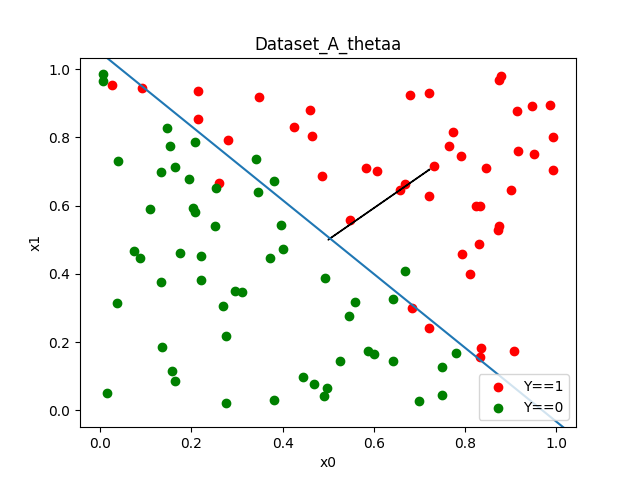
\includegraphics{../src/stability/outputs/Dataset_A_thetaa.png}
\end{figure}
\begin{figure}[H]
	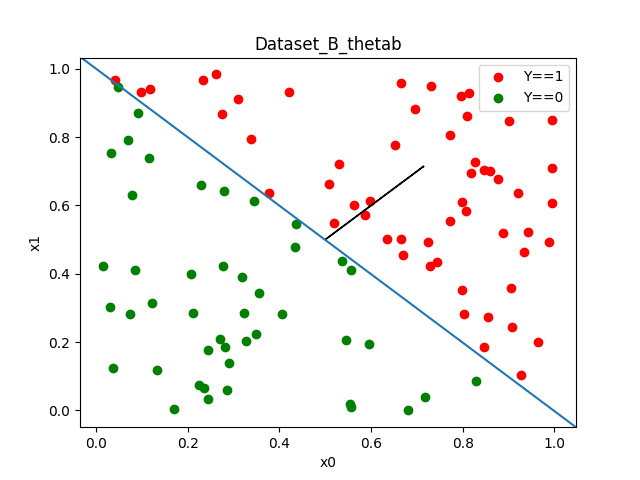
\includegraphics{../src/stability/outputs/Dataset_B_thetab.png}
\end{figure}

We observe that dataset A seems less well differentiated than dataset B, the former has a few points mixing around the boundaries, whereas the latter can almost perfectly be separated by a dividing line. Otherwise the two are very comparable.

The classification line shown are derived many iterations on through gradient descent. For Dataset B we achieve perfect classification, whereas for Dataset A there are a few points that are misclassified, but this is unavoidable. 


\begin{figure}[H]
	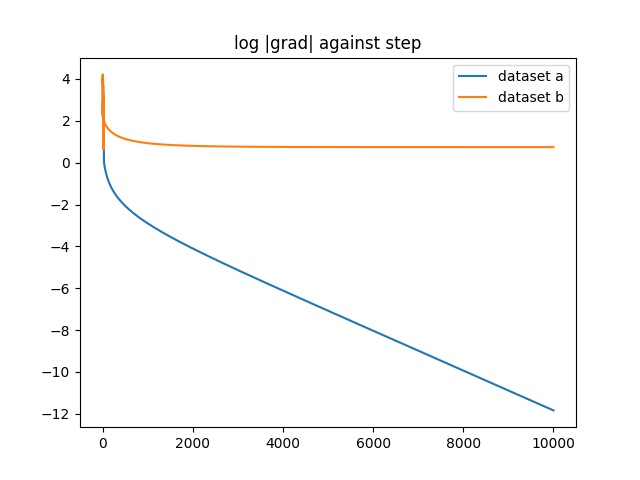
\includegraphics{../src/stability/outputs/log_grad_size.png}
\end{figure}

Our hypothesis is confirmed by this figure which shows the log size of the log likelihood gradient vector, for both they seem to eventually decrease exponentially quickly (linearly in log), but for B it's much shallower a slope than A. This would seem to be because perfect classification is possible with B, such that further improvements can only be made by increasing the magnitude of $\theta$ without changing direction. Indeed if $h_\theta(x) = g(z)$ then $h_{2 \theta}(x) = g(2z)$. If classification is good, then $z >> 0$ or $z << 0$ s.t. writing $e^{-z}=y$, have $g(z) \approx 1-y,\; g(2z) \approx 1 - y^2$ or $g(z) \approx y^{-1},\; g(2z) \approx y^{-2}$, i.e. the size $|y - g(z)|=\epsilon \mapsto \epsilon^2$.

Hence the grad step $\frac{\partial l}{\partial \theta} = \sum (y_i - h_\theta(x_i)) x_i$ roughly gets smaller as we step. I.e. if $\theta \mapsto 2\theta$ then $\epsilon \mapsto \epsilon^2$. I.e. the size of $\frac{\partial l}{\partial \theta}$ is approximately proportional to $\epsilon^{2^k} = \epsilon^{M_k}$ where the parameter $\theta_n$ itself has size $2^k \theta$. The time of doubling, $n_k \propto \theta 2^k \epsilon^{-2^k} \propto M_k \epsilon^{-M_k}$, and so if we roughly map $y = |\text{grad}|$ against $x \approx n_k$, we get a relation like $x \approx \propto M_k/y \approx \propto 1/y$ since $y = \epsilon^{-M_k}$ shrinks much faster than $M_k$ itself. Then $\log | \text{grad} |$ shrinks rather like $- \log x$, i.e. in the long run not like the linear decay we get by dataset A.

That was overly complicated and I'm not even sure if quite correct, but the essence is having no target to aim for size of the gradient slides decreases very slowly, like $1/\text{time step}$, while the parameter itself just gets bigger and bigger (though bigger at a very gradually slowing rate). Some intuition would be better here...
\end{answer}
%\end{document}
} \fi


  \item \subquestionpoints{5}
For each of these possible modifications, state whether or not it would lead to
the provided training algorithm converging on datasets such as $B$. Justify your
answers.
\begin{enumerate}
  \item Using a different constant learning rate.
  \item Decreasing the learning rate over time (e.g. scaling the initial
  learning rate by $1/t^2$, where $t$ is the number of gradient descent
  iterations thus far).
  \item Linear scaling of the input features.
  \item Adding a regularization term $\|\theta\|_2^2$ to the loss function.
  \item Adding zero-mean Gaussian noise to the training data or labels.
\end{enumerate}
 


\ifnum\solutions=1 {
  \begin{answer}
\end{answer}

} \fi


  \item \subquestionpoints{2}
Support vector machines (SVMs) are an alternative machine learning model that we discussed in class.
We have provided you an SVM implementation (using a radial basis function (RBF) kernel) within \texttt{src/spam/svm.py} (You should not need to modify that code).

One important part of training an SVM parameterized by an RBF kernel (a.k.a Gaussian kernel) is choosing an appropriate kernel radius parameter.

Complete the \texttt{compute\_best\_svm\_radius} by writing code to compute the best SVM radius which maximizes accuracy on the validation dataset. Report the best kernel radius you obtained in the writeup.



\ifnum\solutions=1 {
  \begin{answer}
\end{answer}

} \fi

\end{enumerate}
